\chapter{Proposta de um Sistema de Recomendação para Experimentos de ES em LPS}
\label{sec:prop_sis_rec_exp}

Este tópico apresenta a abordagem de um sistema de recomendação para experimentos de ES para LPS.

\section{Objetivos}
\label{sec:obj}

Esta pesquisa tem como objetivo geral em encontrar um sistema de recomendação usando ontologia preditiva em uma base de dados sobre experimentos de software caracterizadas por sua qualidade, a fim de gerar recomendações de processos e diretrizes experimentais para a realização de uma pesquisa experimental em LPS com qualidade.

Neste projeto de pesquisa vamos levantar uma base de dados sobre qualidade de experimentos de ES voltados para LPS. Através dessa base será possível gerar um modelo de dados baseado em ontologias \textbf{TBox} e \textbf{ABox} com o objetivo de extrair informações preditivas desta base. Após processar as informações preditivas baseada nos dados de qualidade de experimentos em ES para LPS, será possível criar um sistema de recomendação, utilizando as ferramentas apropriadas de recomendação em ES, para sistematizar recomendações de projetos experimentais em ES para LPS.

Os objetivos específicos são:

\begin{itemize}
	\item Gerar um conjunto de meta dados das informações sobre experimentos em LPS usando ontologia;
	\item Uma aplicação front-end de interação com usuário afim de gerar recomendações de experimentos em LPS.
\end{itemize}

\section{Metodologia}
\label{sec:meto}

(Papel da ontologia)
Nesta pesquisa será utilizado ontologia para estruturar e modelar a base de informações extraído do Mapeamento Sistemático de experimentos em LPS que está sendo desenvolvido pela pesquisa de dissertação da aluna de mestrado Viviane Furtado.

Pode se dizer que que este modelo será conjunto de meta dados das informações extraídas da pesquisa de dissertação da Viviane Furtado.

O processo de execução deste trabalho para chegar ao objetivo será, pesquisar de maneira exploratória um modelo de sistema de recomendação em experimentos de ES para LPS. Para tal resultado será desenvolvido um projeto de software e em seguida executar este projeto.

O processo de desenvolvimento do projeto de software, inclui realizar a escolha das tecnologias a serem usadas como ferramenta de construção do software, como por exemplo, as linguagens de programação, o ambiente de desenvolvimento, a diagramação do projeto, os \textit{stakeholders} envolvidos no projeto, ferramentas de Application Lifecycle Management (ALM) aplicadas ao escopo do projeto, escolha das abordagens de sistemas de recomendação, definição do modelo de ontologias, definição da base de dados para representação tanto dos dados de origem (itens, usuários) para recomendação como representação dos dados para apresentação e armazenamento dos resultados obtidos da recomendação. 

Após a definição do projeto de software, inicia-se o processo desenvolvimento do sistema de recomendação. Com o auxílio de ferramentas de ALM todos os \textit{stakeholders} envolvidos será possível acompanhar o desenvolvimento online da ferramenta, desta forma se tornando um processo mais colaborativo entre eles. 
Inicialmente será realizado a modelagem dos dados extraído da avaliação de qualidade dos experimentos de ES em LPS realizado pelo trabalho da Viviane Furtado, que são mais de 100 experimentos encontrado na literatura nesse ramo de pesquisa. Em seguida será aplicado um modelo de ontologia definido no projeto de software nesta base de informações de experimentos com o propósito de realizar predições para um modelo mais abstrato sobre qualidade de experimentos em ES em LPS. Na sequência será desenvolvido o modelo de recomendação modelado na fase de projeto de software, esse desenvolvimento consiste na modelagem dos dados encontrado na predição da ontologia para extrair as informações necessárias para o modelo de recomendação, posteriormente aplicar os algoritmos neste modelo. A última fase desse desenvolvimento será a criação de um \textit{front-end} de interação com o usuário no sistema de recomendação.


\section{Avaliação}
\label{sec:aval}
Na Literatura é possível encontrar algumas dimensões para avaliação de um sistema de recomendação e as recomendações provida por ele. Em \cite{robillard2010recommendation} são apresentadas 16 dimensões de avaliação para um sistema de recomendação em ES que estão apresentadas na subseção a seguir. Cada uma dimensão possui sua técnica de avaliação, algumas são quantitativas outras qualitativas e algumas possuem as duas abordagens.

\paragraph*{Corretude}
Quão próximo é a recomendação do conjunto de recomendações que assumimos ser corretas?

\paragraph*{Cobertura}
Até que ponto a cobertura do SR sobre um conjunto de itens ou o espaço do usuário?

\paragraph*{Diversidade}
Qual a diversidade das recomendações?

\paragraph*{Confiável}
Como a recomendação pode ser confiável?

\paragraph*{Confiança do SR}
Quão confiante o SR é?

\paragraph*{Novidade}
Qual é o sucesso do SR em gerar novas recomendações ou recomendações ainda desconhecidas para o usuário?

\paragraph*{Acaso}
Até que ponto o SR ainda promove surpresa com sucesso?

\paragraph*{Utilidade}
Qual é o ganho de valor dessa recomendação para o usuário?

\paragraph*{Risco}
Qual é o risco para o usuário aceitar essa recomendação?

\paragraph*{Robustez}
Qual é a tolerância do SR para um viés ou uma informação falsa?

\paragraph*{Taxa de Aprendizagem}
Quão rápido é o SR para adicionar novas informações ou atualizar a lista de recomendação?

\paragraph*{Usabilidade}
O qual usável é o SR? Será fácil dos usuários de adequar de uma forma apropriada?

\paragraph*{Escalabilidade}
Quão escalável é o SR em relação ao numero de usuários, levando em consideração o tamanho dos dados e a performance dos algoritmos?

\paragraph*{Estabilidade}
Quão consistente é o SR em um período de tempo?

\paragraph*{Privacidade}
Existe algum risco a privacidade do usuário?

\paragraph*{Preferência do usuário}
Como o usuário entende o SR?

Essas dimensões podem ser subdivididas em categorias como mostra a \ref{tab:dimens-catg}. As dimensões centradas na recomendação avaliam principalmente as recomendações geradas pelo próprio sistema de recomendação. As dimensões centradas no usuário nos permitem avaliar se o sistema de recomendação atende às necessidades do seu usuário final. As dimensões centradas no sistema, em contraste, fornecem principalmente formas de avaliar o próprio sistema de recomendação, ao invés das recomendações ou da perspectiva do usuário. Finalmente, as dimensões centradas na entrega são principalmente o foco do sistema de recomendação no contexto do uso \cite{robillard2010recommendation}.


\begin{table}[]
	\centering
	\caption{Categorização das 16 dimensões. Tradução de \cite{robillard2010recommendation}}
	\label{tab:dimens-catg}
	\begin{tabular}{@{}llll@{}}
		\toprule
		\begin{tabular}[c]{@{}l@{}}Centralizado na \\ Recomendação\end{tabular} & \begin{tabular}[c]{@{}l@{}}Centralizado no \\ Usuário\end{tabular} & \begin{tabular}[c]{@{}l@{}}Centralizado no \\ Sistema\end{tabular} & \begin{tabular}[c]{@{}l@{}}Centralizado na \\ Entrega\end{tabular} \\ \midrule
		Corretude & Confiável & Robustez & Usabilidade \\
		Cobertura & Novidade & Taxa de Aprendizagem & Preferência do usuário \\
		Diversidade & Acaso & Escalabilidade &  \\
		Confiança do SR & Utilidade & Estabilidade &  \\
		& Risco & Privacidade &  \\ \bottomrule
	\end{tabular}
\end{table}

\section{Contribuições}
\label{sec:contr}

Espera-se que com este trabalho seja encontrado uma modelo (projeto e implementação) de recomendação experimentos de ES para LPS, focado em potencializar a qualidade do experimento a ser recomendado. Espera-se também realizar um estudo de caso a fim de analisar o modelo proposto.

Espera-se que com esta pesquisa inicie um processo de melhoramento na qualidade de experimentação em LPS através deste projeto e implementação do sistema de recomendação proposto.

\section{Trabalhos Futuros}
\label{sec:trab-fut}

Como trabalho futuro espera-se desenvolver melhores abordagens de recomendação afim de comparação com a abordagem proposta.

\section{Limitações}
\label{sec:limit}

Uma possível limitação deste estudo é o tempo hábil para implementação e testes de
validação do sistema de recomendação.

\section{Cronograma}
\label{sec:cron}

As etapas que compõem o cronograma de execução desta proposta de projeto de dissertação de mestrado são descritas a seguir e apresentadas abaixo e na \ref{fig:cronograma} evidenciado as que estão em andamento, a serem executadas e conclu??das de acordo com legenda informada no final desta Seção


\begin{itemize}
	\item E1 - RSL - Revisão sistemática da Literatura
	\item E2 - Projeto: Tecnologias
	\item E3 - Projeto: Modelo de Ontologias
	\item E4 - Projeto: Modelo de Predição
	\item E5 - Projeto: Modelagem de dados
	\item E6 - Projeto: Modelo de Recomendação
	\item E7 - Projeto: Front-End
	\item E8 - Desenvolvimento: Ontologias
	\item E9 - Desenvolvimento: Predição
	\item E10 - Desenvolvimento: Recomendação
	\item E11 - Desenvolvimento: Front-End
	\item E12 - Testes
	\item E13 - Avaliação dos Resultados
	\item E14 - Conclusões
	\item E15 - Escrever Qualificação
	\item E16 - Defesa da Qualificação
	\item E17 - Escrever Dissertação
\end{itemize}

\begin{figure}[htb]
	\centering					
	{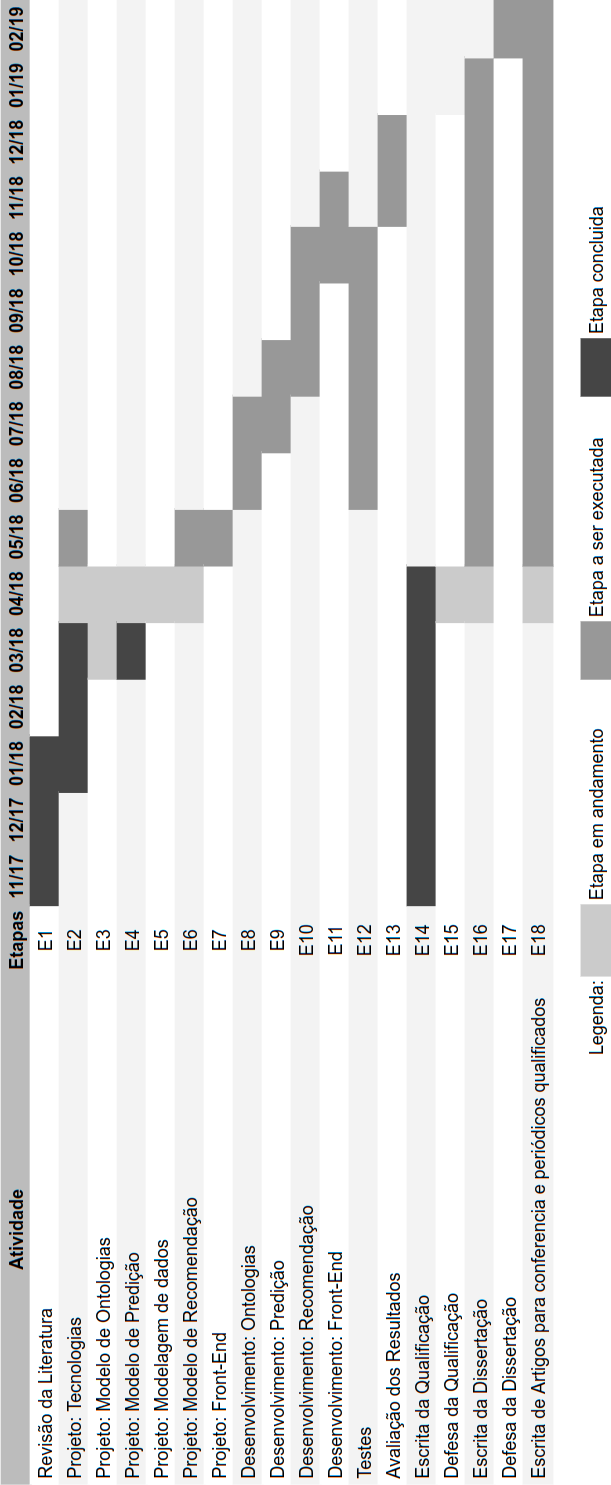
\includegraphics[scale=.4]{cronograma.png}}
	
	\caption{Conceitos Essenciais de um Experimento. Traduzido de Wohlin et al. (2012)}
	\label{fig:cronograma}
\end{figure}
